%These are end of chapter provblems for the student to try. They should be in an exercise environment.
\section{Past Paper Problems}

\begin{exercise} %N16HLP1-Q2
	State the purpose of cache memory.
	\begin{solution}
		It is used to save time in accessing RAM
	\end{solution}
\end{exercise}
	
\begin{exercise} %N16HLP1-Q2
Draw a diagram to show the relationship between random access memory (RAM), the processor and cache memory.
\begin{solution}
	Here is the diagram.\\
	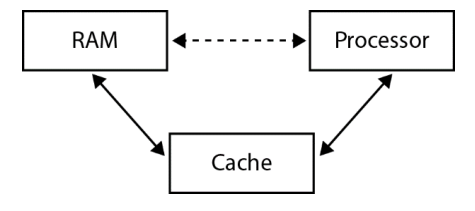
\includegraphics[scale=0.5]{topic_1_systems/topic_1_exercises/RAMdiagram}	
\end{solution}
\end{exercise}

\begin{exercise*} %N16HLP1-Q8
A book shop has a computer at each point of sale, and also a central computer. When a customer buys a book in the book shop, the salesperson at the point of sale uses a scanning device to input a barcode from the book. The barcode is sent to the central computer where the barcode of each book and the corresponding price are held in a database on a disk.
When the price is found, it is sent to the point of sale computer where all necessary calculations are performed, details of the transaction are stored on a local disk and a receipt is printed out.
\begin{parts}
	\item Construct a system flow chart for the system described above.
	\newline
	At the point of sale there are peripheral devices other than the scanning device and printer.
	\item Outline the purpose of one other possible peripheral device in this scenario.
	
\begin{solution}
\newline
Keyboard;
To type in some additional data;
Or to type in barcode data when it is not possible to scan;

Magnetic card reader;
Used when a credit card is used;

Microphone;
To call the next customer;
To call manager;

Monitor;
So the salesman can see the information/data on the screen;

Visual display;
So the customer can read the information/data on the display;

Speakers;
For customers to hear information;
For shop assistants to bring another item the customer may wish to buy
\end{solution}
\end{parts}
\end{exercise*}	
	